\section{IAU2018}

%\frame
%{
%%...................................................................................................
%\note<1>[]{}
%%...................................................................................................
%	\frametitle{}
%	\begin{itemize}
%		\item 
%	\end{itemize}
%	\centering
%%	\includegraphics[width=115mm]{images/}
%}

\frame[t]
{
%...................................................................................................
\note<1>[]{}
%...................................................................................................
	\frametitle{\alert{T}otal \alert{S}olar \alert{I}rradiance}
	\begin{itemize}
		\item TSI -- spectrally integrated solar radiative flux at 1 AU from the sun \\
	\end{itemize}

	\centering
	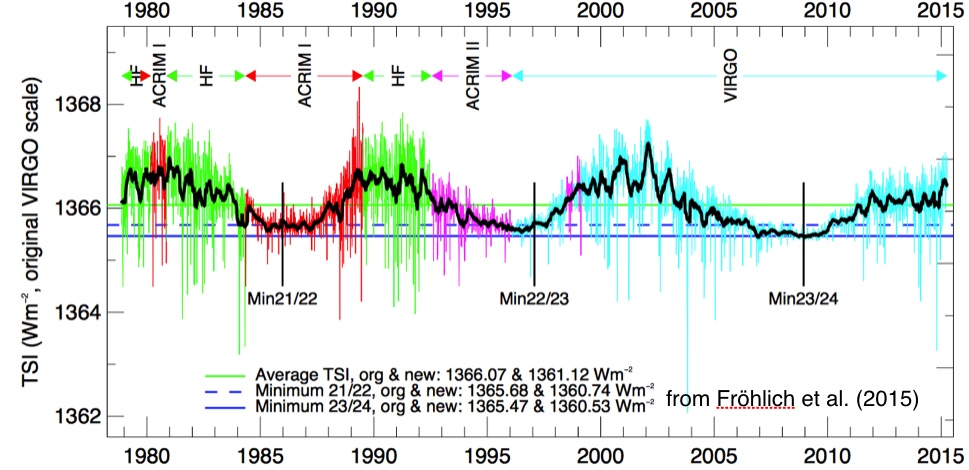
\includegraphics[width=\textwidth]{images/tsi}
	
}


\frame
{
%...................................................................................................
\note<1>[]{}
%...................................................................................................
	\frametitle{Spectra of the individual components}
	\centering
	Solar spectra \\
	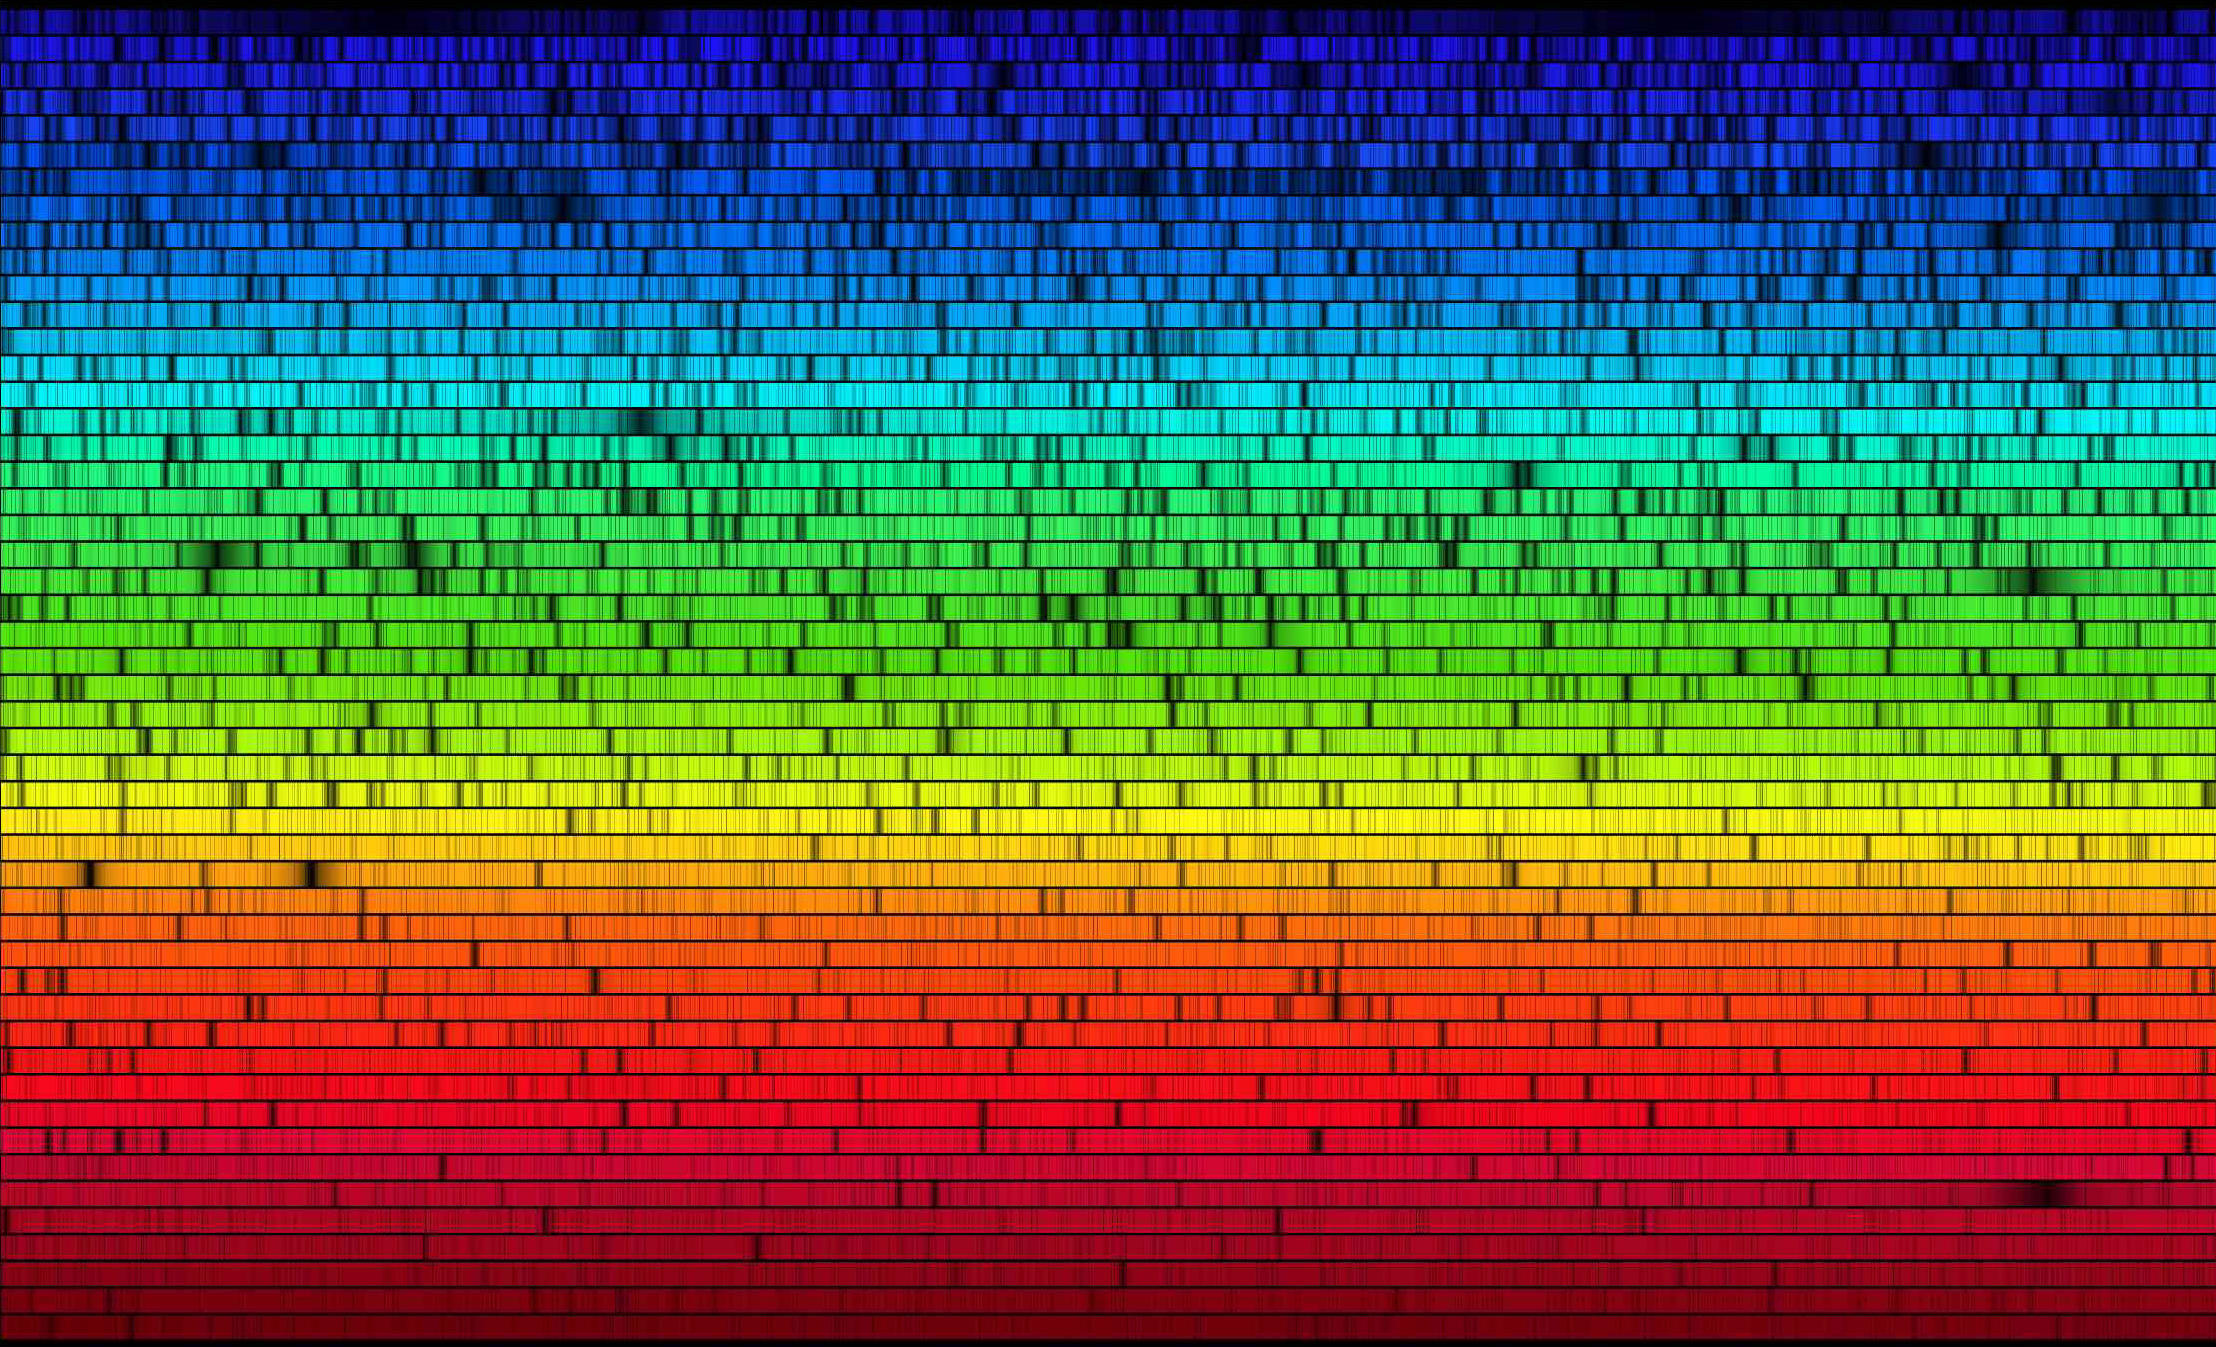
\includegraphics[width=.9\textwidth]{images/solar_spectra}
	
}



\frame[t]
{
%...................................................................................................
\note<1>[]{}
%...................................................................................................
	\frametitle{Importance of lines for variability}
	\begin{itemize}
		\item TSI -- \alert{T}otal \alert{S}olar \alert{I}rradiance, i.e. integrated over wavelengths
		\item SSI -- \alert{S}pectral \alert{S}olar \alert{I}rradiance, depends on wavelength 
		\item $\triangle$ -- difference between the solar minima and maxima
		%\item The increase of the TSI at maximum of the activity cycle compared with minimum is directly attributed to the variability in spectral lines
	\end{itemize}
	\centering
	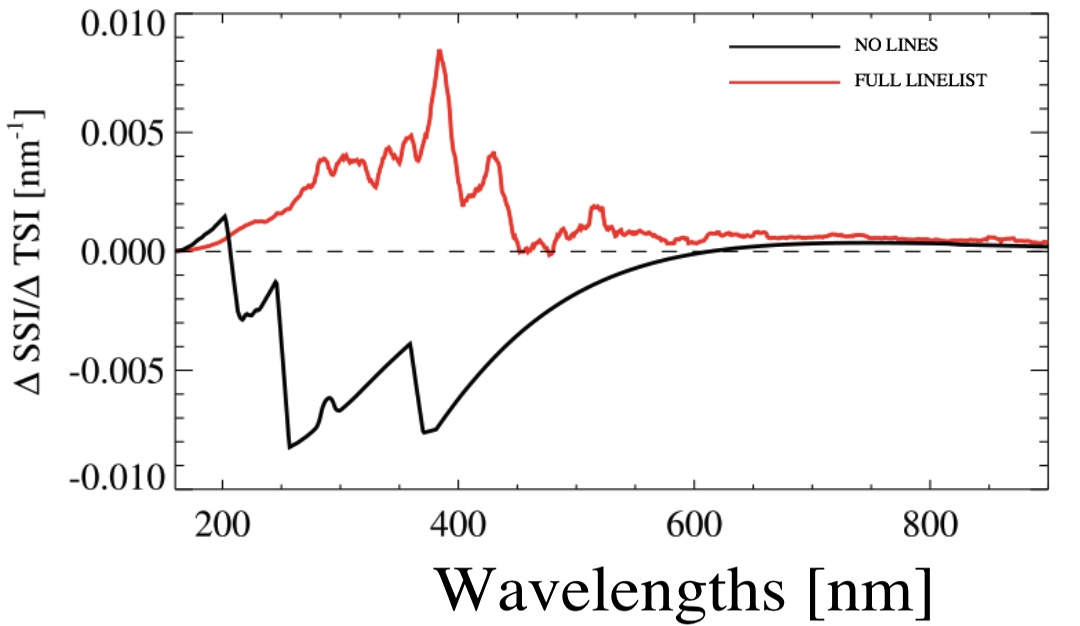
\includegraphics[width=90mm]{images/continuum}
}


%\frame[t]
%{
%%...................................................................................................
%\note<1>[]{}
%%...................................................................................................
%	\frametitle{Importance of lines for variability}
%	\vspace{3em}
%	\centering
%	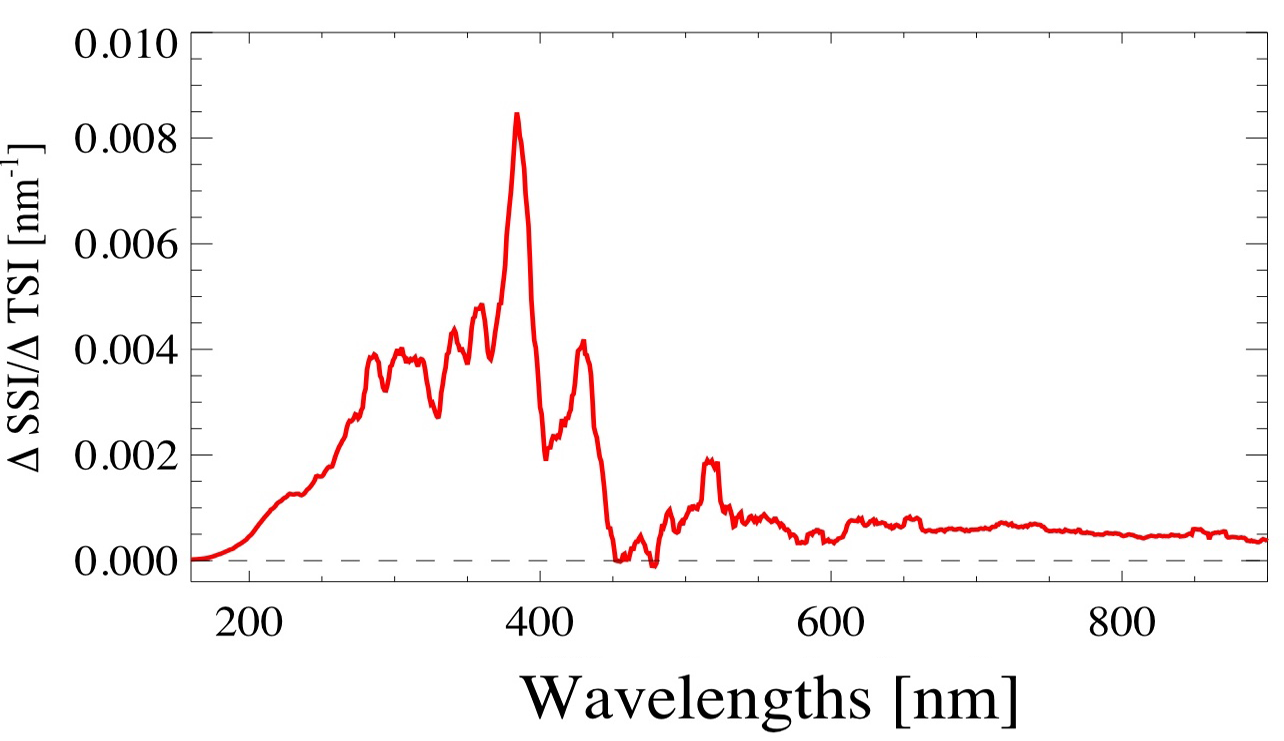
\includegraphics[width=90mm]{images/timescales_1}
%}

\frame[t]
{
%...................................................................................................
\note<1>[]{}
%...................................................................................................
	\frametitle{Importance of lines for variability}
	\vspace{3em}
	\centering
	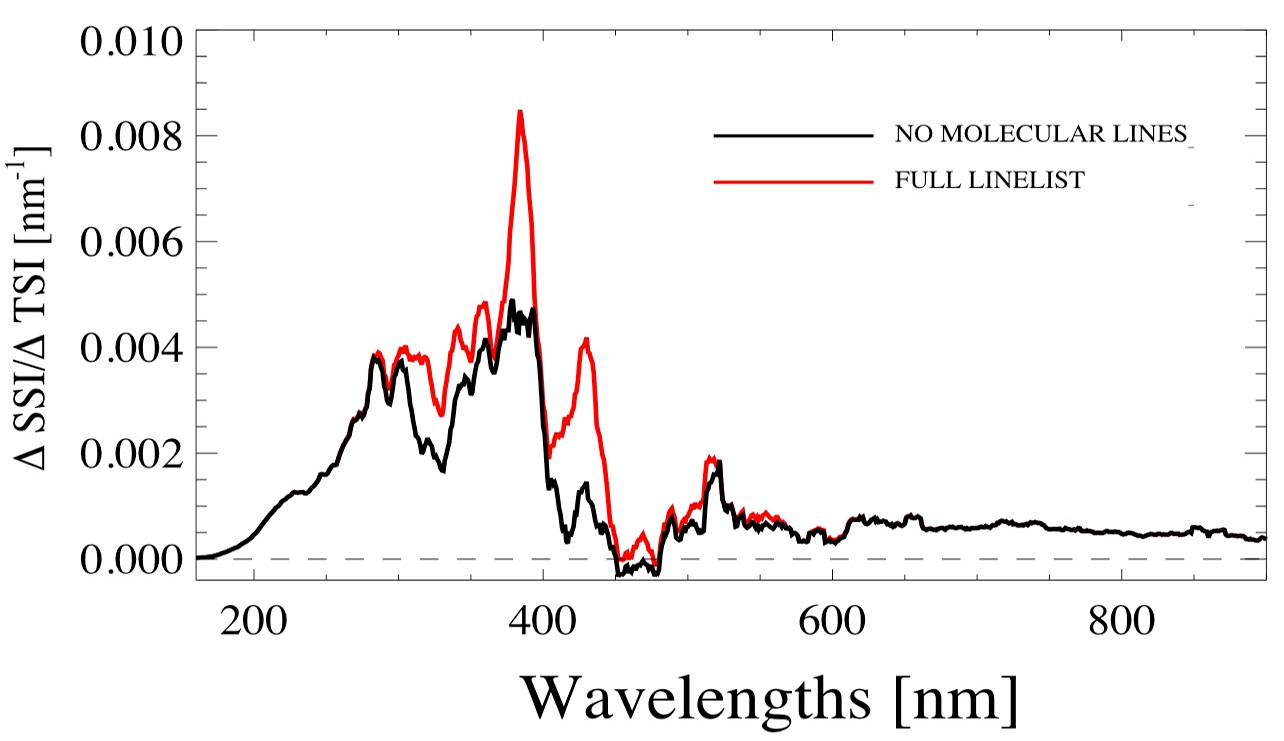
\includegraphics[width=.9\textwidth]{images/timescales_2}
}


\frame[t]
{
%...................................................................................................
\note<1>[]{}
%...................................................................................................
	\frametitle{Importance of lines for variability}
	\begin{itemize}
		\item<2-> \alert{25\%} of the variability comes from molecular lines $\rightarrow$ accurate linelists are required
	\end{itemize}
	\centering
	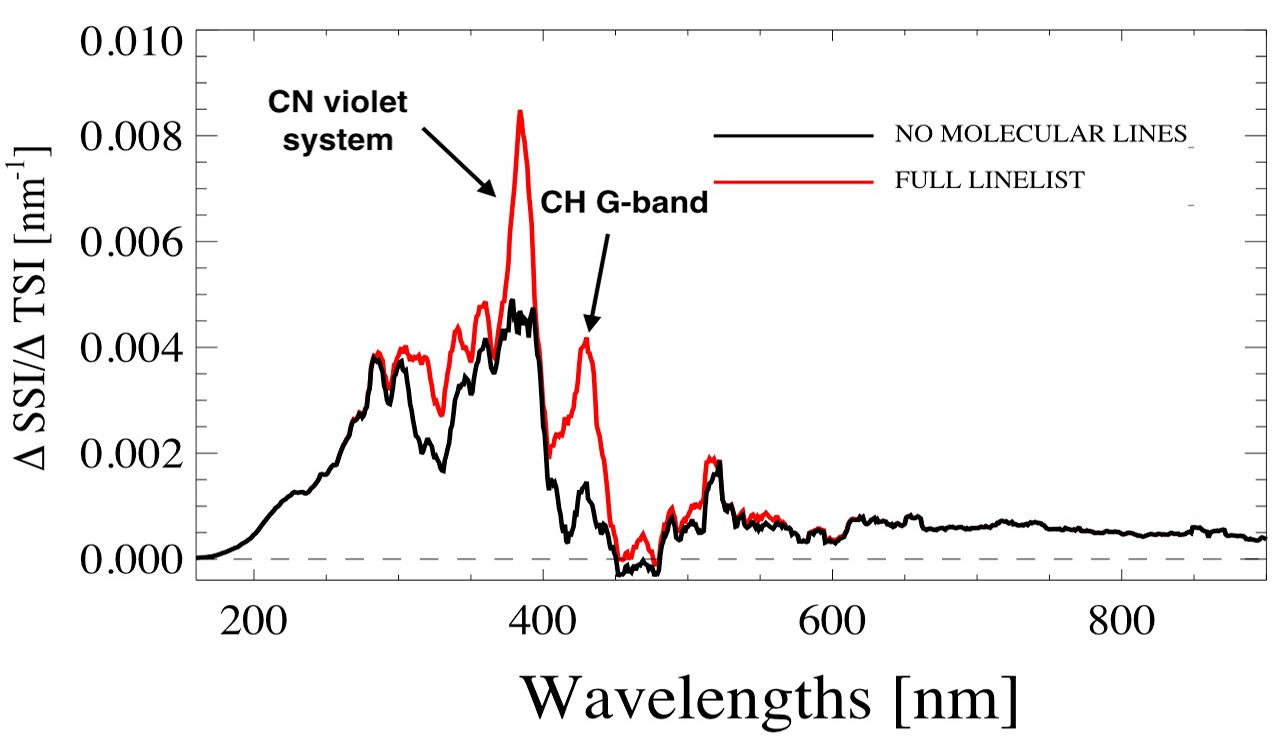
\includegraphics[width=.9\textwidth]{images/timescales_3}
}

\frame
{
%...................................................................................................
\note<1>[]{}
%...................................................................................................
	\frametitle{1.5D simulations}
	\centering
	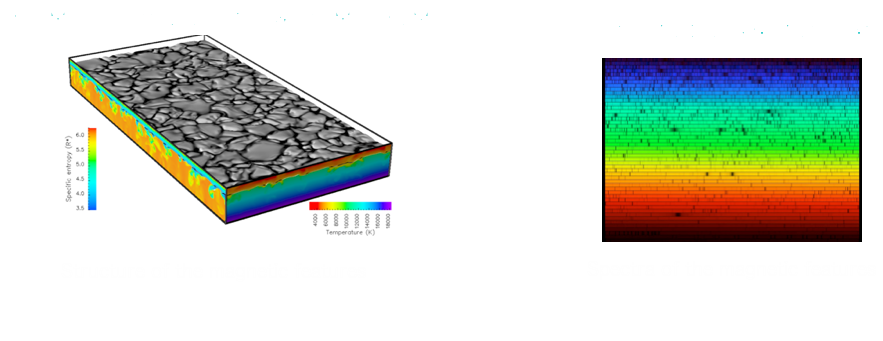
\includegraphics[width=115mm]{images/1_5D}
}



%\frame
%{
%%...................................................................................................
%\note<1>[item]{The Str\"omgren filters B and Y, as well as the Kepler passband or the COROT filter, are broadly used for observations.
%
%Therefore, these filters are of particular interest when radiative transfer calculations are performed. Currently, this is computationally demanding due to a huge amount of atomic and molecular lines.
%
%In this talk, I will show that a SIGNIFICANT speed up can be achieved by using optimized opacity detribution functions, which we call OODF!
%
%Let’s start with the example of the Strömgren Y filter. As you can see the intensity is dominated by lines….}

\frame
{
%...................................................................................................
\note<1>[]{}
%...................................................................................................
	\frametitle{Generating ODFs}
	\begin{itemize}
    \item Start with high resolution opacity	
	\end{itemize}

	\centering
	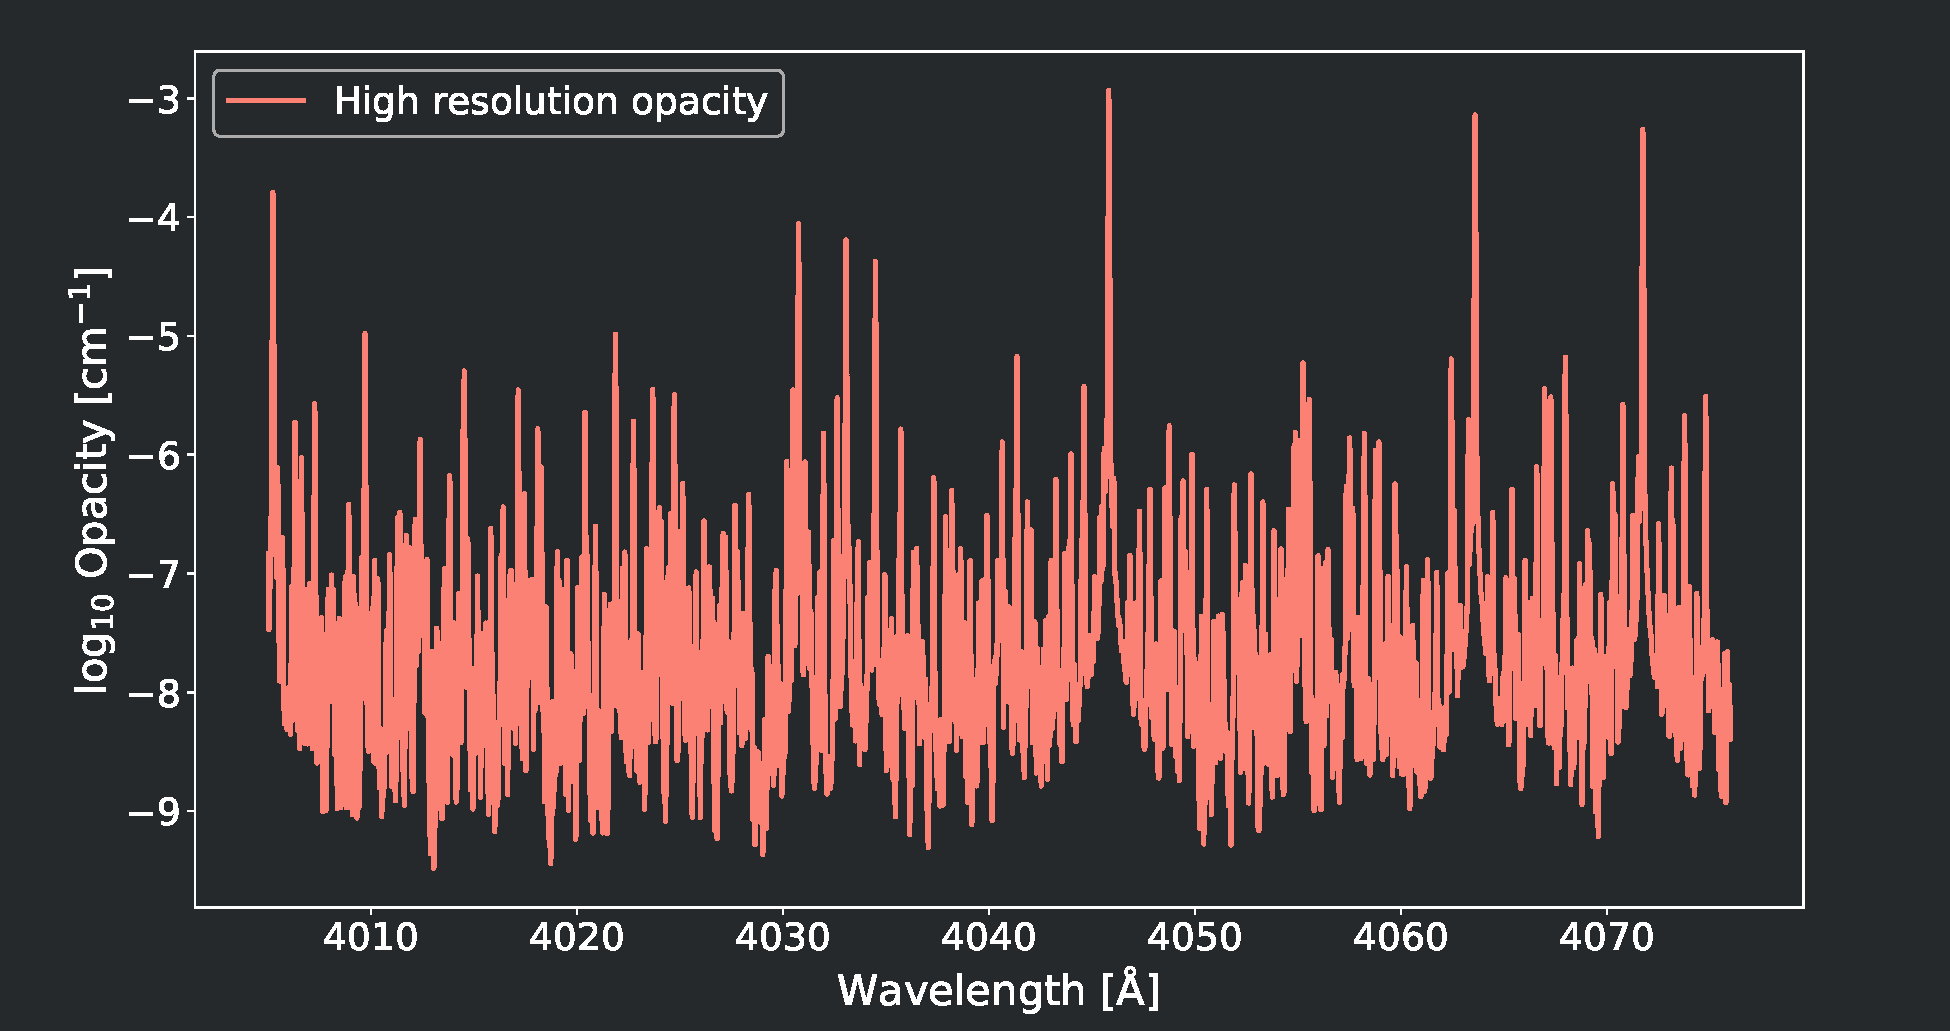
\includegraphics[width=115mm]{images/odf_generation_process_0}
}

\frame
{
%...................................................................................................
\note<1>[]{}
%...................................................................................................
	\frametitle{Generating ODFs}
	\begin{itemize}
    \item Sort wavelength points by corresponding values of opacity; monotonically increasing opacity
    \item Integral is preserved by sorting
	\end{itemize}		
	\centering
	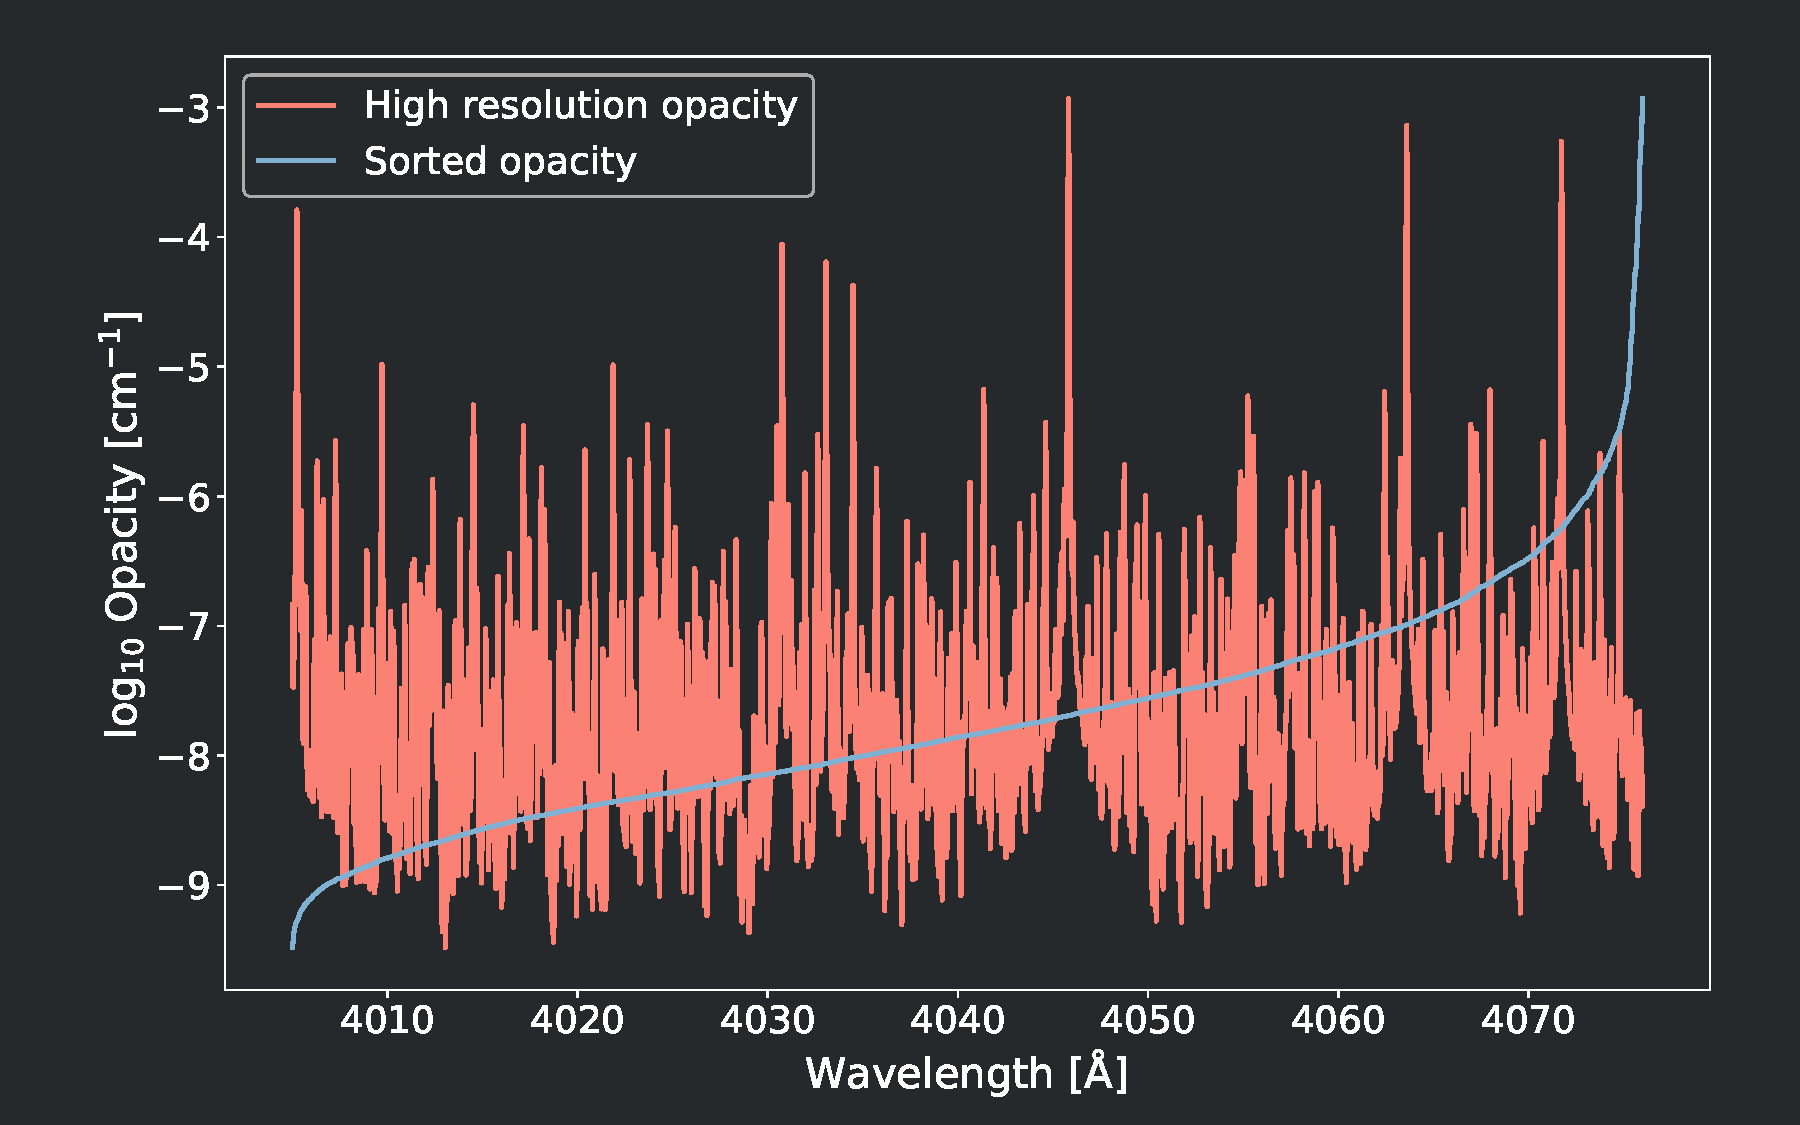
\includegraphics[width=108mm]{images/odf_generation_process_1}
}

\frame
{
%...................................................................................................
\note<1>[item]{Take notes here.}
%...................................................................................................
	\frametitle{Generating ODFs}
	\begin{itemize}
		\item All wavelength information within the bin is lost
\end{itemize}		

		\centering
	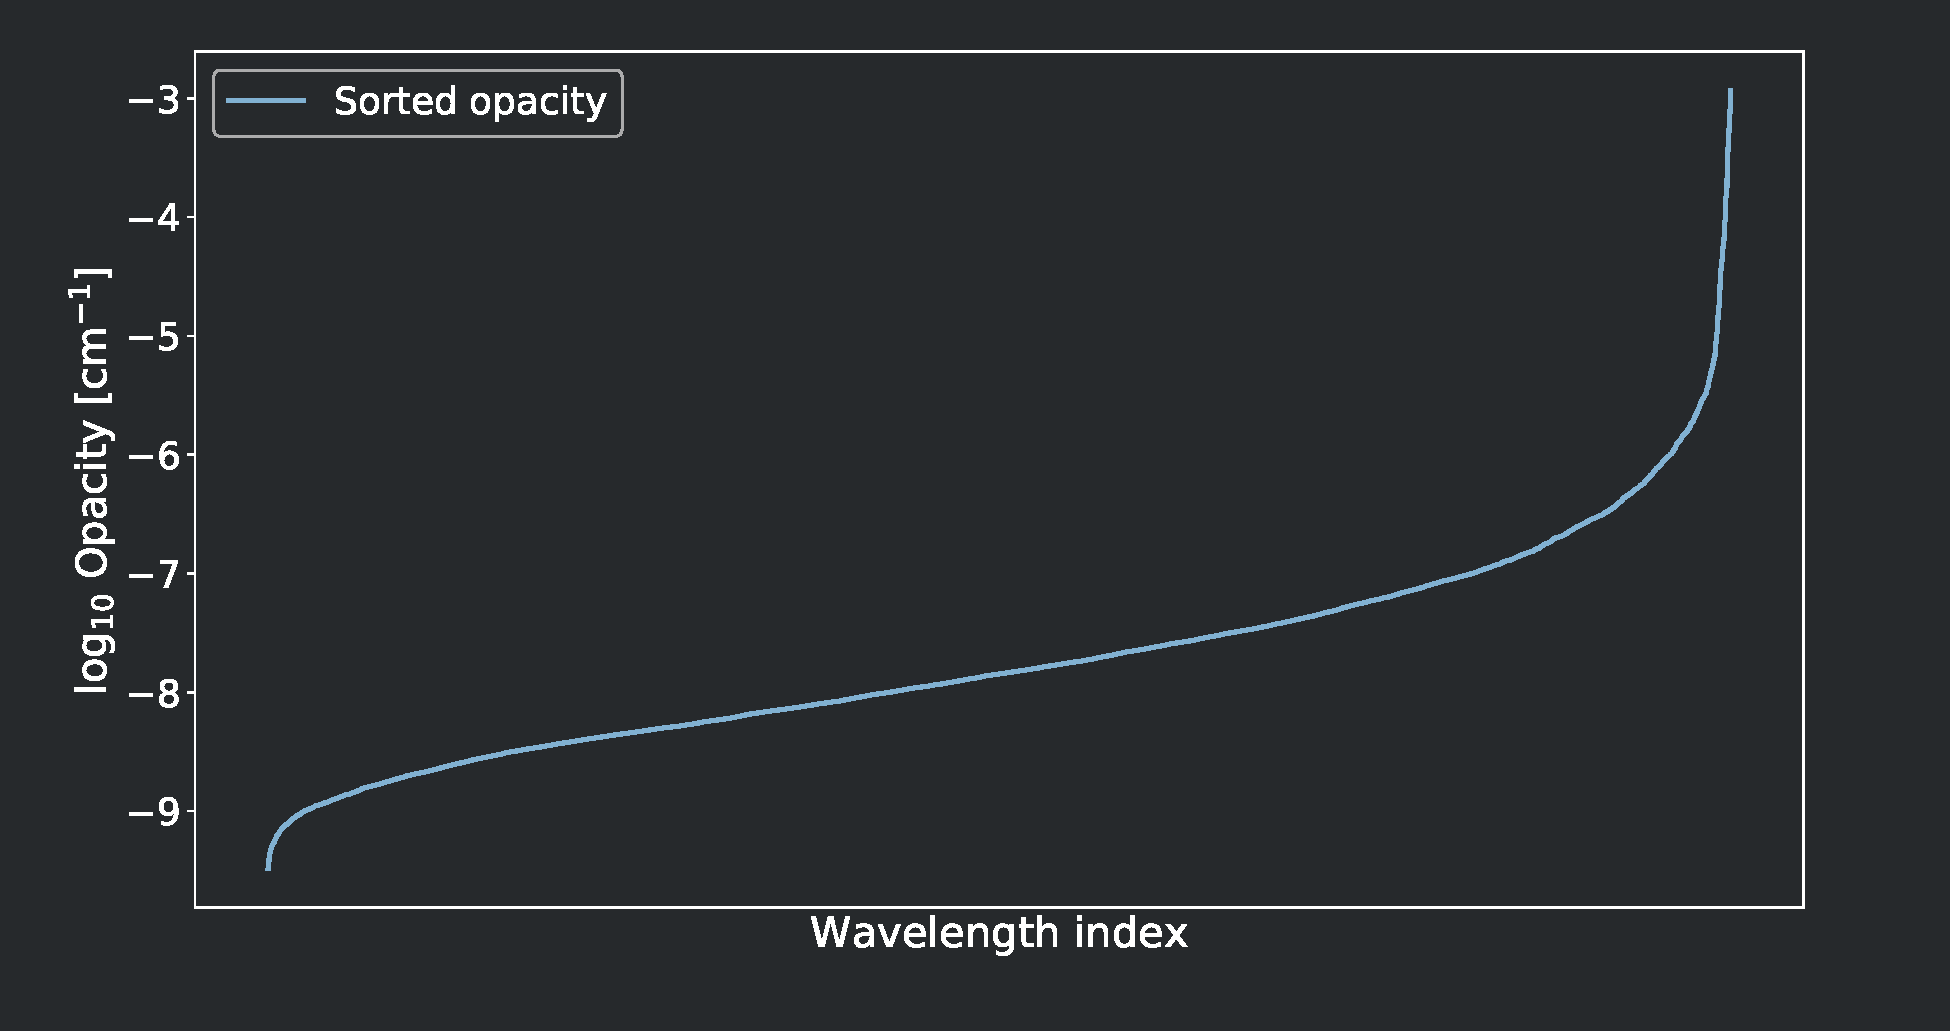
\includegraphics[width=115mm]{images/odf_generation_process_2}
}

\frame
{
%...................................................................................................
\note<1>[]{}
%...................................................................................................
	\frametitle{Generating ODFs - Example with 10 uniform sub bins}
	\begin{itemize}
		\item Approximate the sorted opacity with a step-wise function
	\end{itemize}
	\centering
	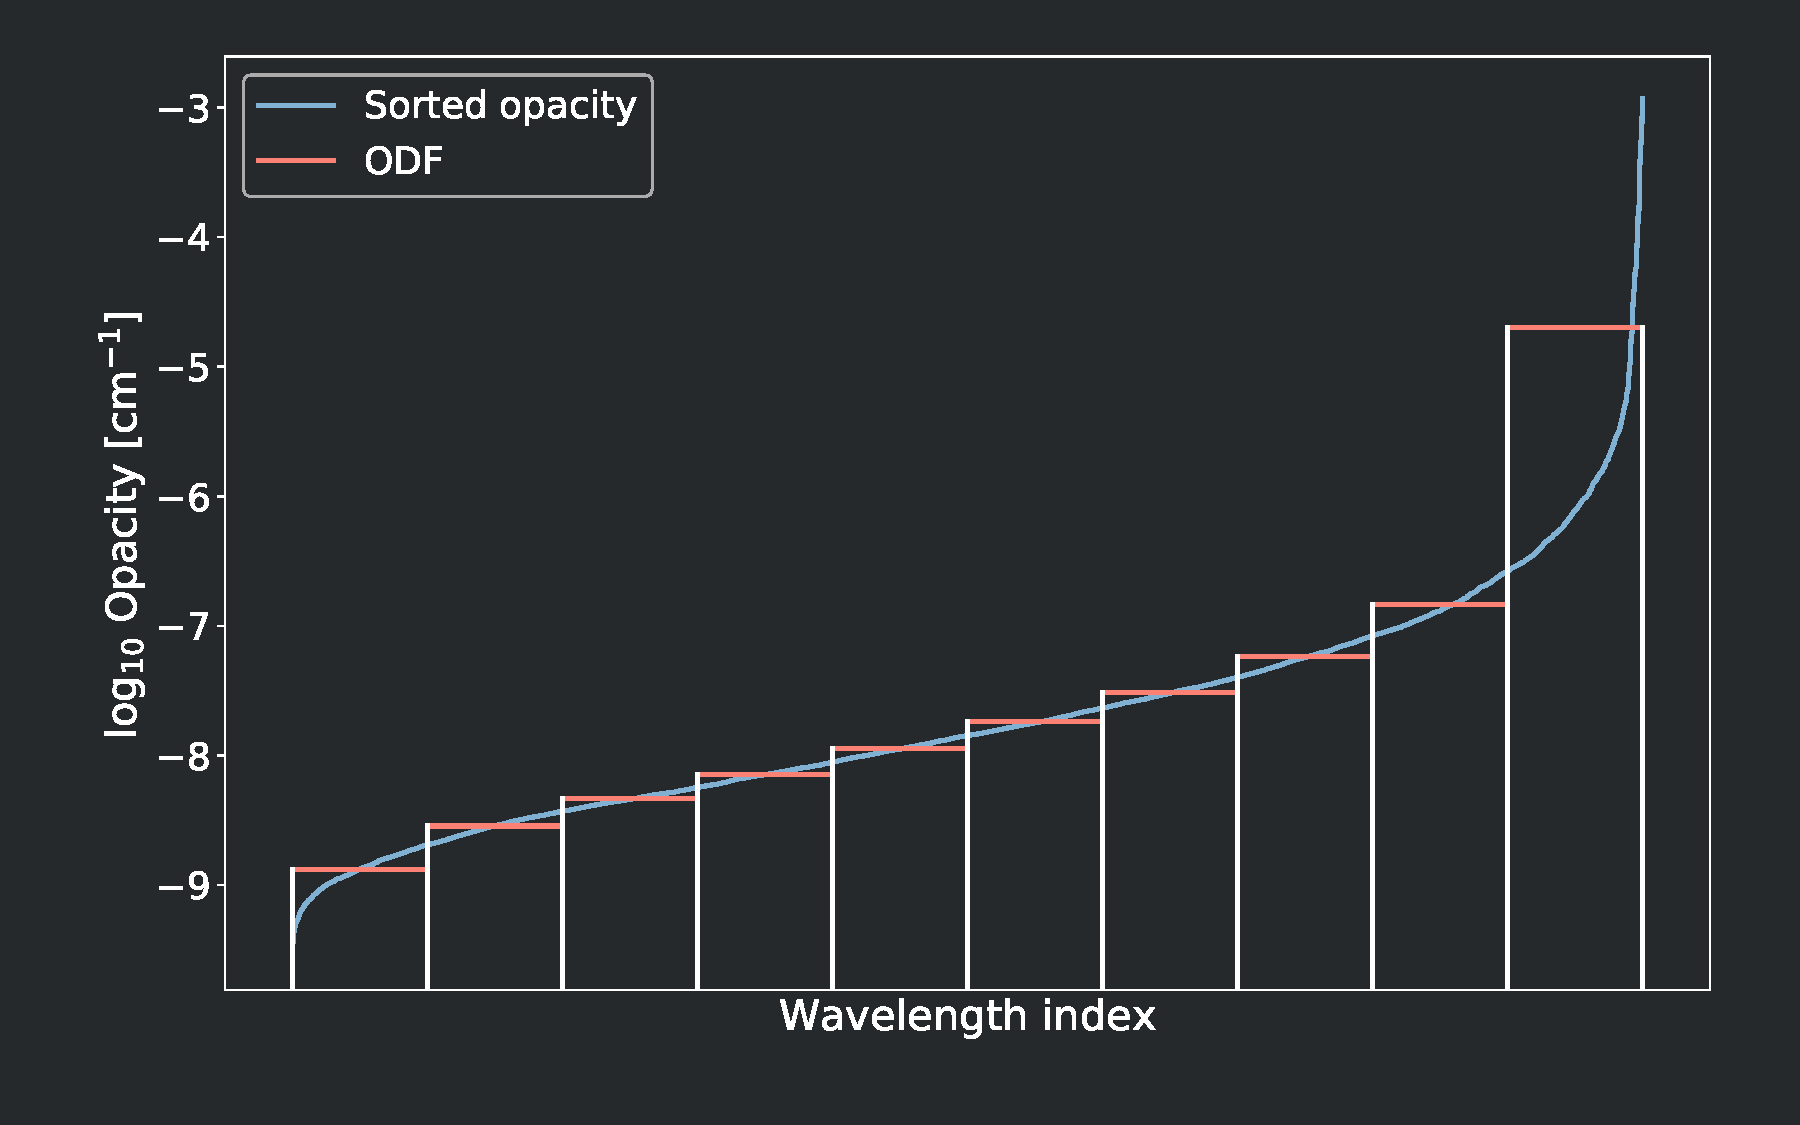
\includegraphics[width=115mm]{images/odf_generation_process_3}
}
\frame
{
%...................................................................................................
\note<1>[]{}
%...................................................................................................
	\frametitle{ODF generation process}
	\begin{itemize}
	\item Mean is skewed by extreme values
	\end{itemize}
	\centering
	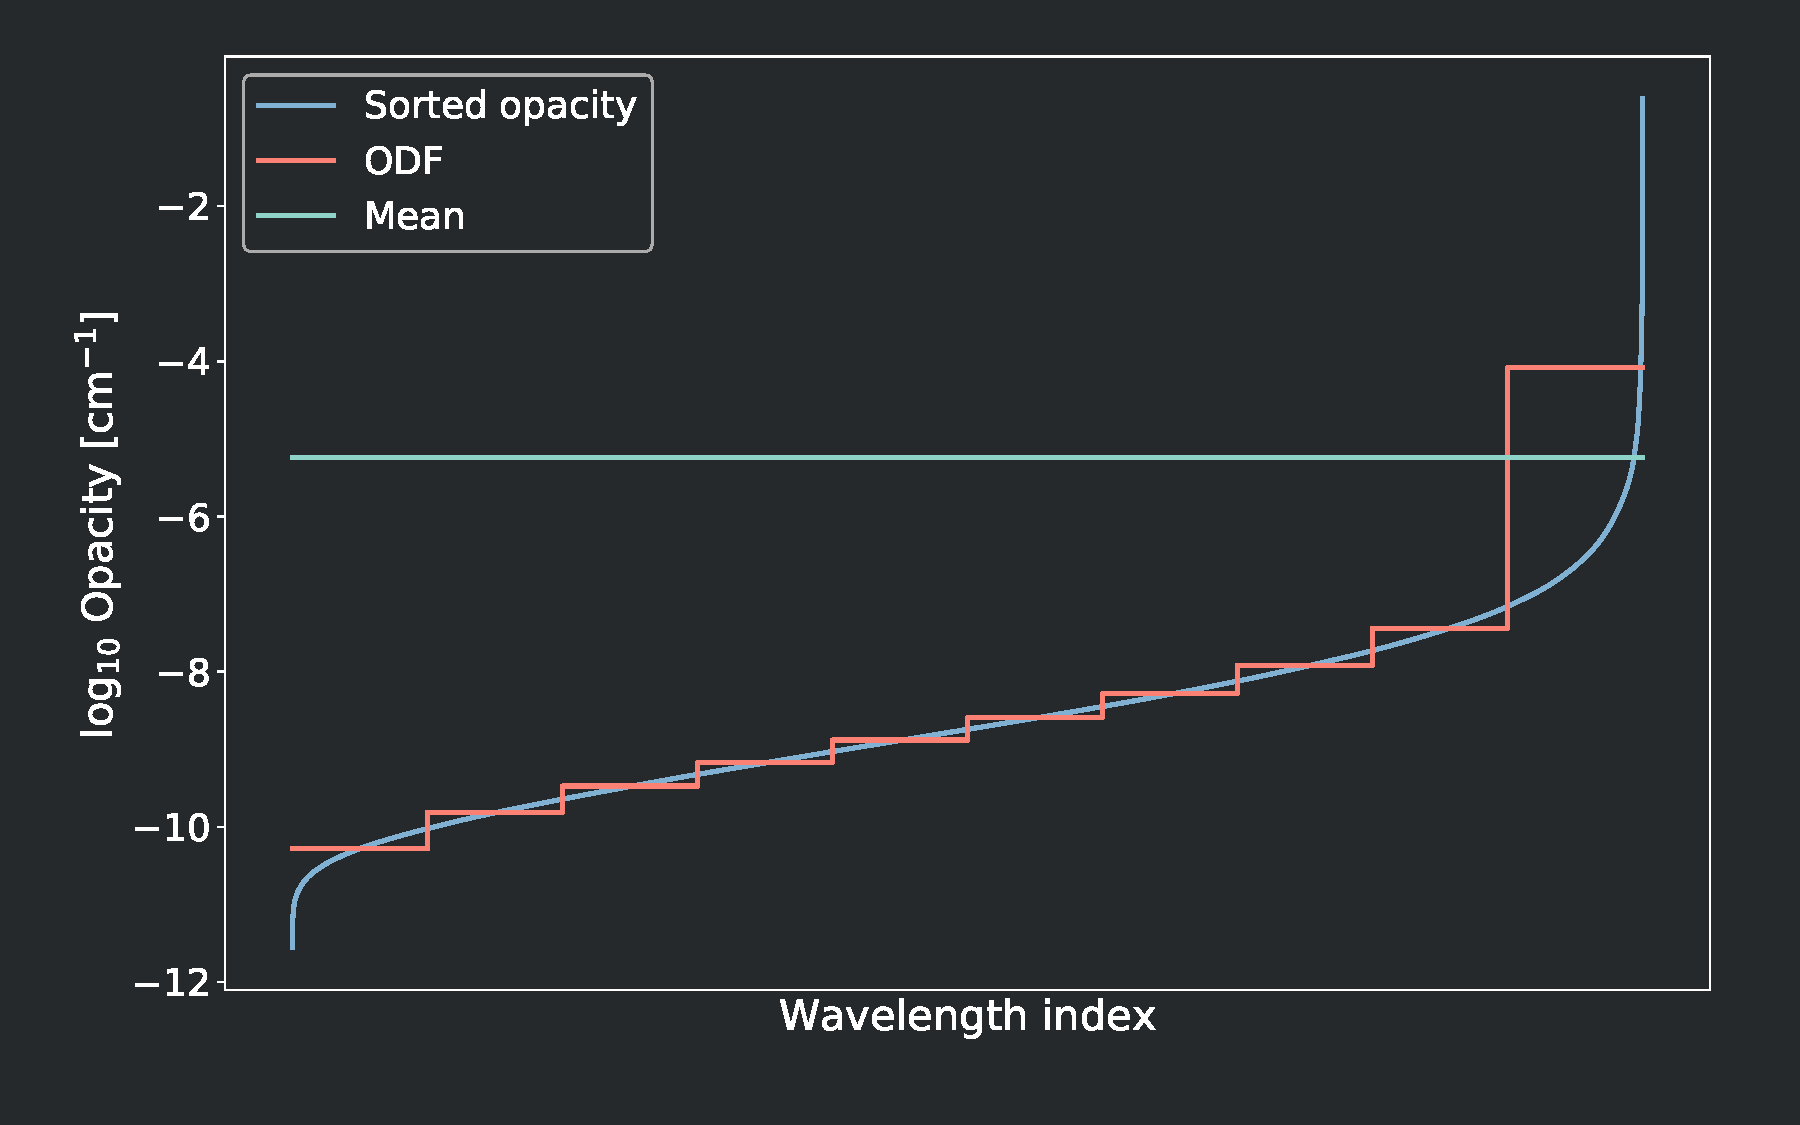
\includegraphics[width=115mm]{images/odf_generation_process_4}
}

\frame
{
%...................................................................................................
\note<1>[]{}
%...................................................................................................
	\frametitle{ODF performance analysis}
	\begin{itemize}
	    \item Synthesize spectrum using ODFs from 1000-9000\si{\angstrom} with 10\si{\angstrom} bins
	    \item Compare the fluxes from the ODF spectrum with the high resolution spectrum in the bins
	\end{itemize}
	\centering
	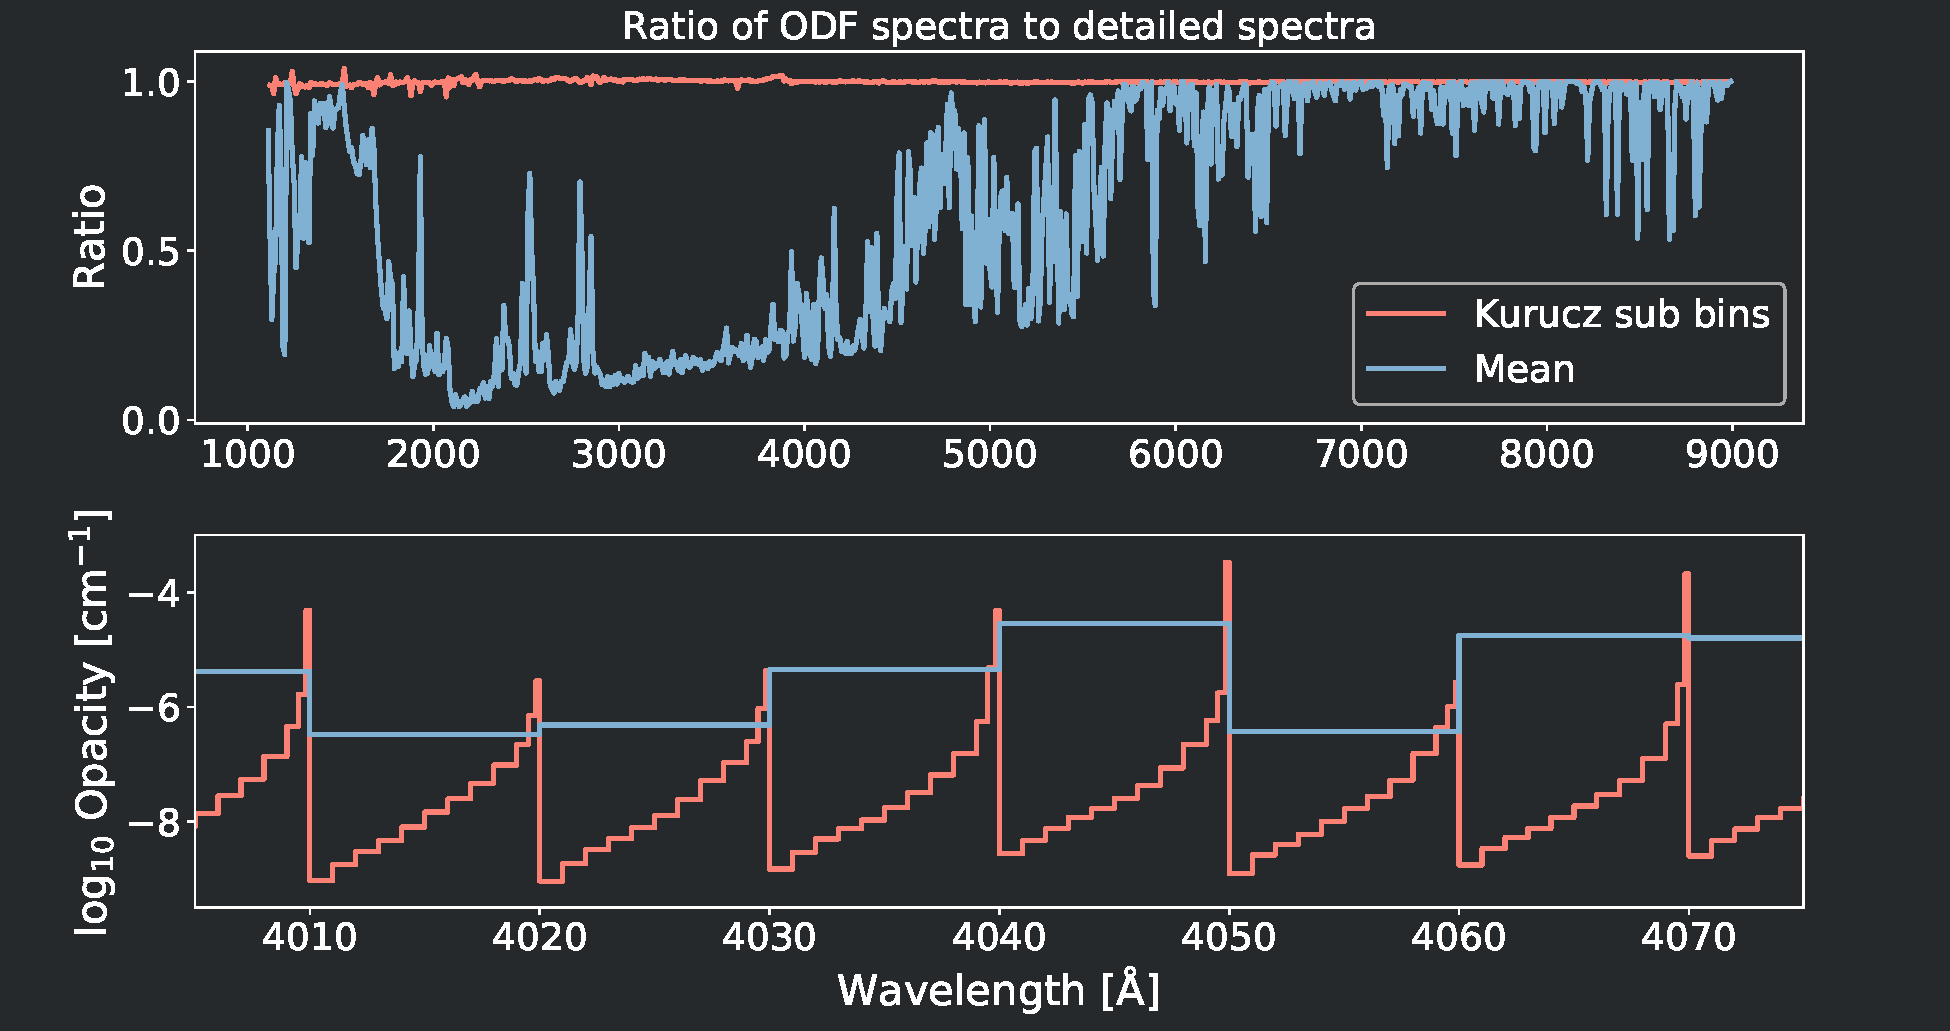
\includegraphics[width=111mm]{images/odf_vs_non_odf}
}


\frame[t]
{
%...................................................................................................
\note<1>[]{}
%...................................................................................................
	\frametitle{Possible solutions}
	Number of calculations goes as: \large{$n_{bins} \times n_{sub bins}$ }
	\vspace{1.6em}
	
	\centering
	
\begin{tikzpicture}[sibling distance=25em,
  every node/.style = {shape=rectangle, rounded corners,
    draw, align=center, color=white!20}]]
  \node {\Large{what to do?}}
    child { node {increase bin size \\
    				  $\rightarrow$ decrease $n_{bins}$} }
    child { node {decrease the number\\ of sub bins per bin} };
\end{tikzpicture}

%	\includegraphics[width=115mm]{images/}
}


\frame
{
%...................................................................................................
\note<1>[item]{}
%...................................................................................................
	\frametitle{Analysis of different ODFs}
	\begin{itemize}
	\item Uniform ODFs
	\end{itemize}
	
	\centering
	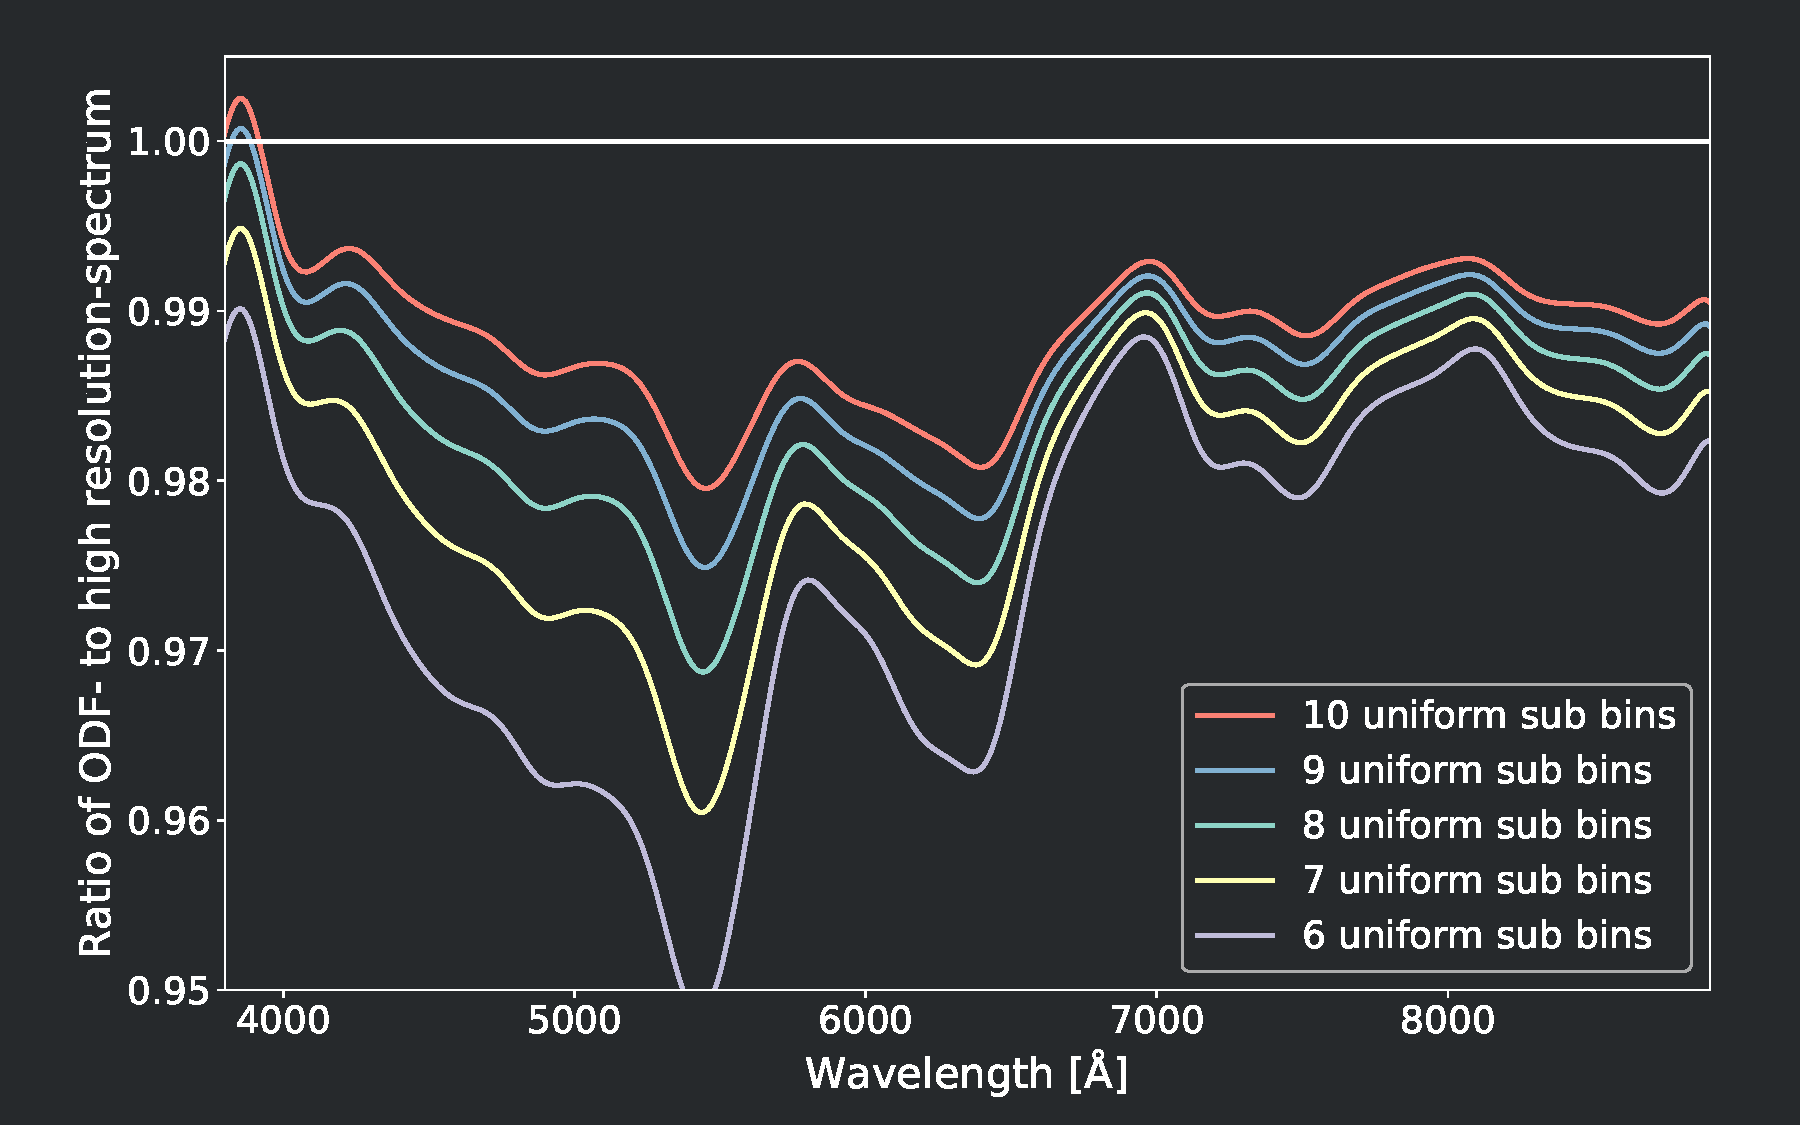
\includegraphics[width=115mm]{images/6_10_vs_best_4_0}
}
\frame
{
%...................................................................................................
\note<1>[]{}
%...................................................................................................
	\frametitle{Analysis of different ODFs}
	\begin{itemize}
		\item Nonuniform ODFs
		\item The last sub bin is crucial after 5000\si{\angstrom}
    \end{itemize}	  
	\centering
	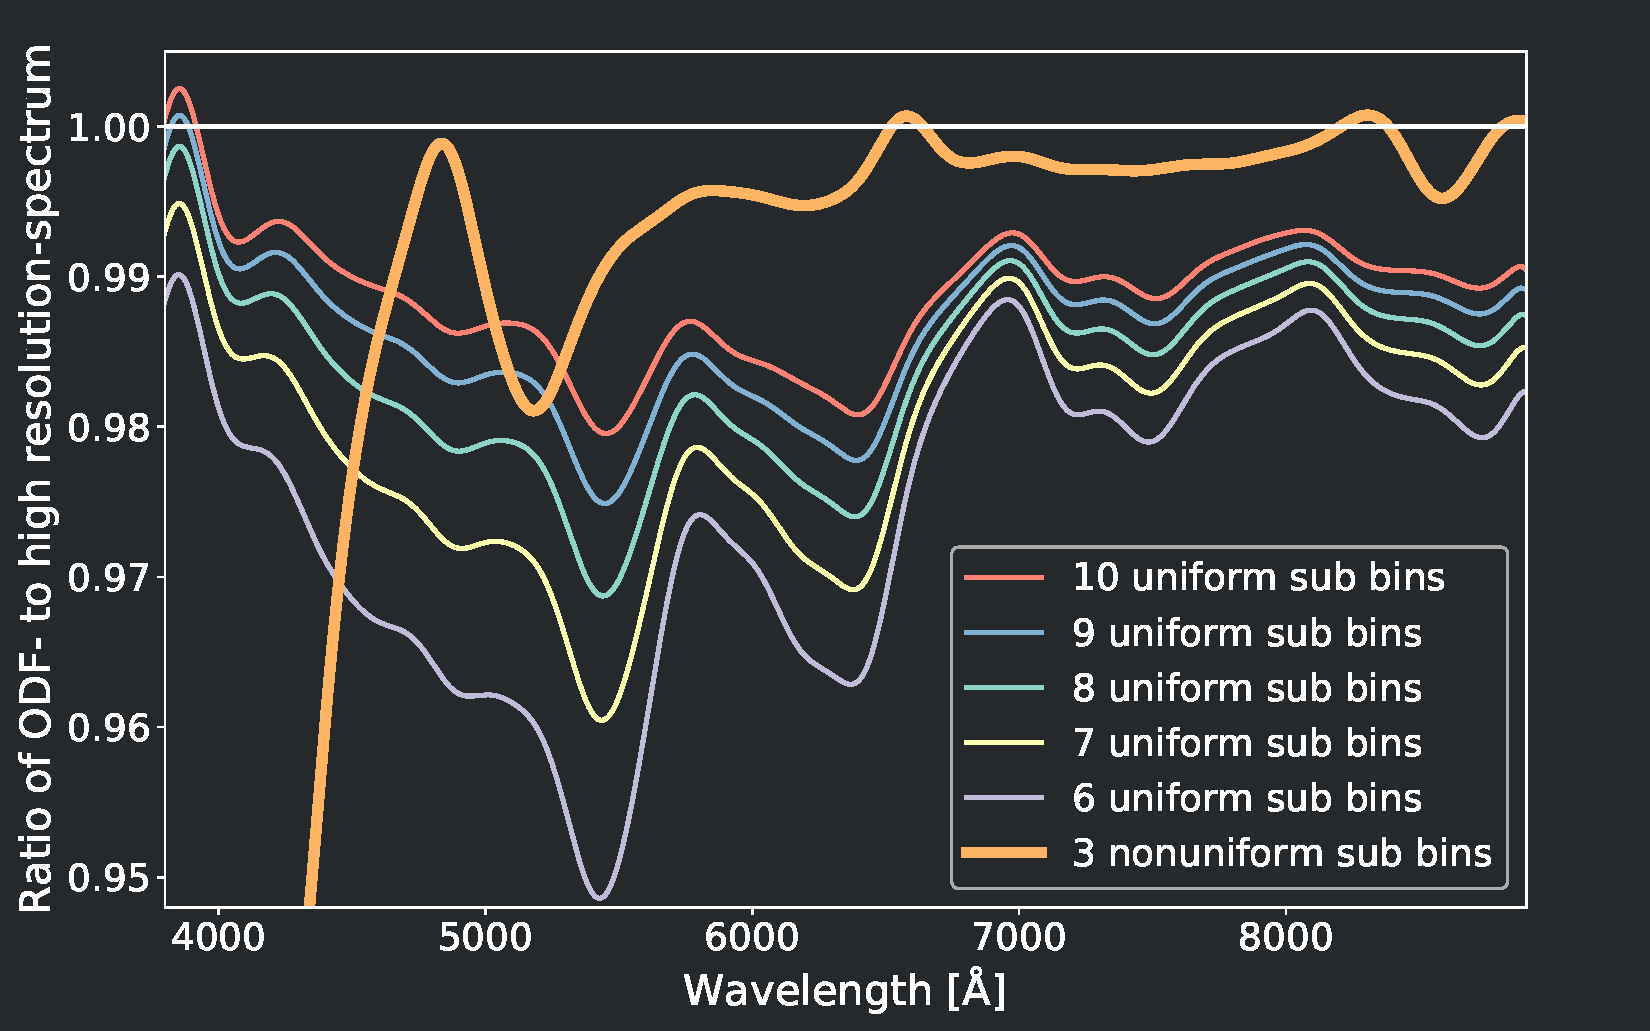
\includegraphics[width=115mm]{images/6_10_vs_best_4_1}
}
%\frame
%{
%%...................................................................................................
%\note<1>[]{}
%%...................................................................................................
%	\frametitle{Comparison of nonuniform sub bins}
%	\begin{itemize}
%	    \item Legend specifies sub bin sizes, starting with the first one
%	    \item Last sub bin is the same for all
%	\end{itemize}
%	\centering
%	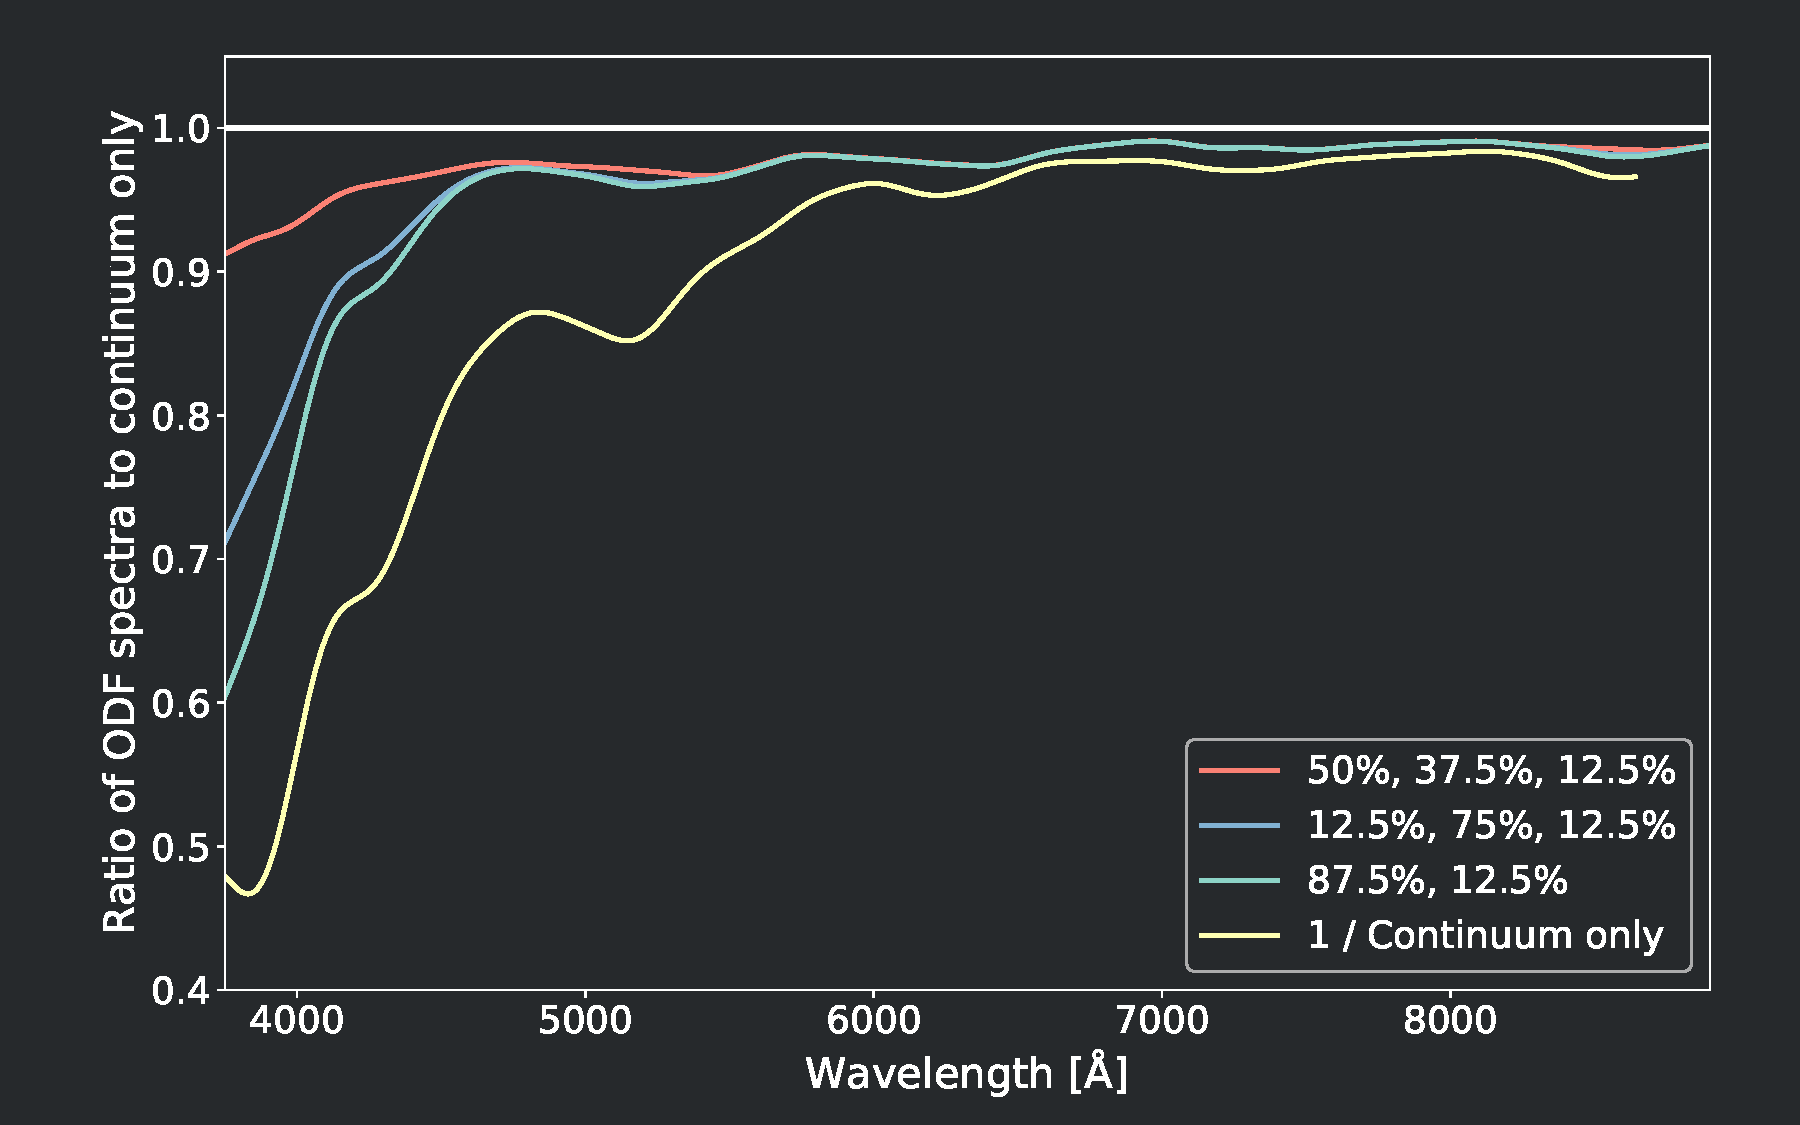
\includegraphics[width=111mm]{images/same_last_sub_bin}
%}
\frame
{
%...................................................................................................
\note<1>[]{}
%...................................................................................................
	\frametitle{Best sub bin combinations using 4 sub bins}
	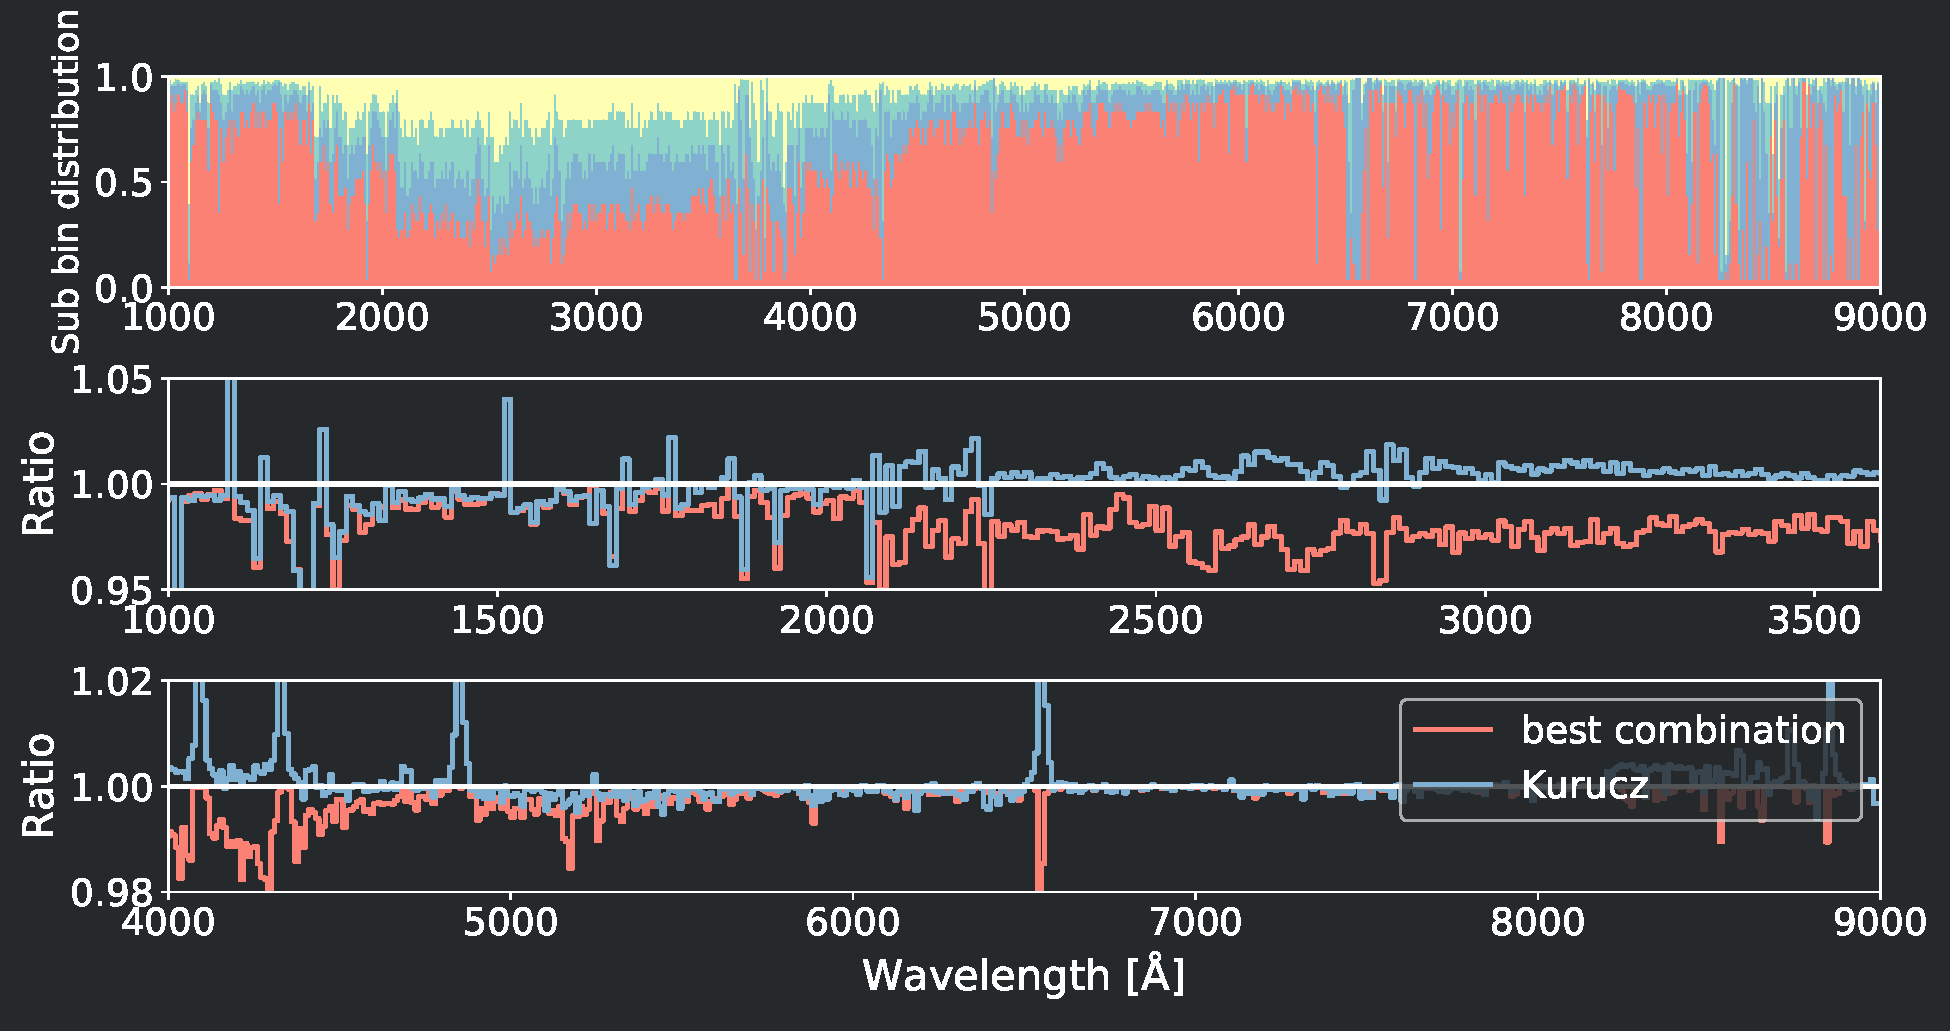
\includegraphics[width=125mm]{images/best_combination_finder_0}
}
\frame
{
%...................................................................................................
\note<1>[]{}
%...................................................................................................
	\frametitle{Best combination of 4 sub bins for Str\"omgren b}
	\begin{itemize}
		\item Total line contribution $\sim$15\%
	\end{itemize}
	\centering
	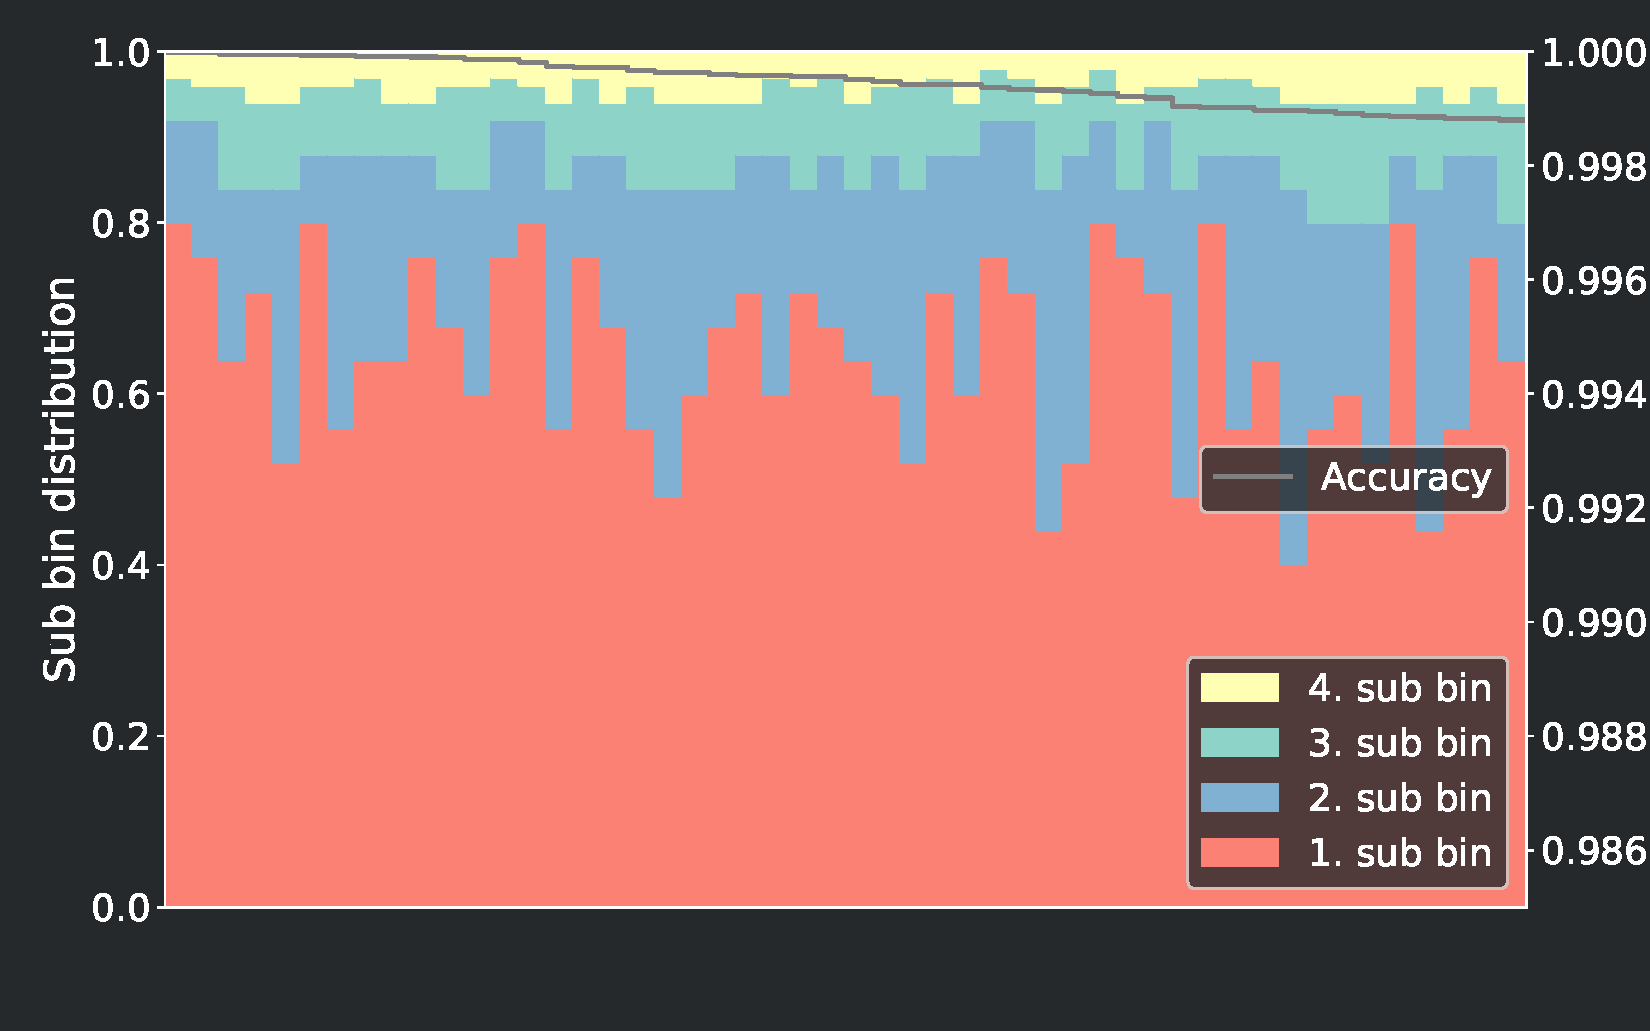
\includegraphics[width=115mm]{images/optimal_stroemgren_1_c_b}
}

\frame
{
%...................................................................................................
\note<1>[]{}
%...................................................................................................
	\frametitle{Speedups in the case of Str\"omgren \textit{b}}
	\begin{itemize}
		\item Interval length: $\sim$400\si{\angstrom}\\[20pt]
	\end{itemize}
	
	\centering
%	High resolution calculation 80 points per \si{\angstrom} $\sim$ 80 000 \\
%	ODF calculations 12 points per 10\si{\angstrom} $\sim$ 1200 \\
%	OODF calculations 3 points per 1000\si{\angstrom} $\sim$ 3 \\

\begin{tikzpicture}[sibling distance=25em,
  every node/.style = {shape=rectangle, rounded corners,
    draw, align=center, color=white!20}]]
  \node {\large{High resolution: 80 points per \si{\angstrom} $\sim$ 32 000 points}\\}
    child { node {ODF: 12 points per 10\si{\angstrom} $\sim$ 480 points \\
    \alert{\large{speedup 67 times}}} }
    child { node {OODF: 3 points for the whole bin\si{\angstrom} $\sim$ 3 points \\
    \alert{\large{speedup $\sim$11 000 times}}} };
\end{tikzpicture}

}

\frame
{
%...................................................................................................
\note<1>[]{}
%...................................................................................................
	\frametitle{Conclusions}
	\large{
	\begin{itemize}
	%\item An efficient  procedure for radiative transfer is timely for new generation of solar and stellar variability models.\\[15pt]
	\item We developed a novel method for fast spectral synthesis. \\[15pt]
	\item Found optimal sub bins for different wavelength regimes.\\[15pt]
    \item Can be tailored for different filters: Strömgren \textit{b} + \textit{y}, Kepler, PLATO  and others.\\[15pt]
    \item Significant speed up relative to standard  methods by a factor of at least two orders of magnitude.\\[10pt]
	\end{itemize}
	
	}
	\pause
		\centering \alert{\Large{Thank you for your attention!}} \\
		\pause
		
\includegraphics[width=25mm]{images/qr}
}


\frame
{
%...................................................................................................
\note<1>[]{}
%...................................................................................................
	\frametitle{Best combinations of 4 sub bins for Str\"omgren \textit{b}}
	\centering
	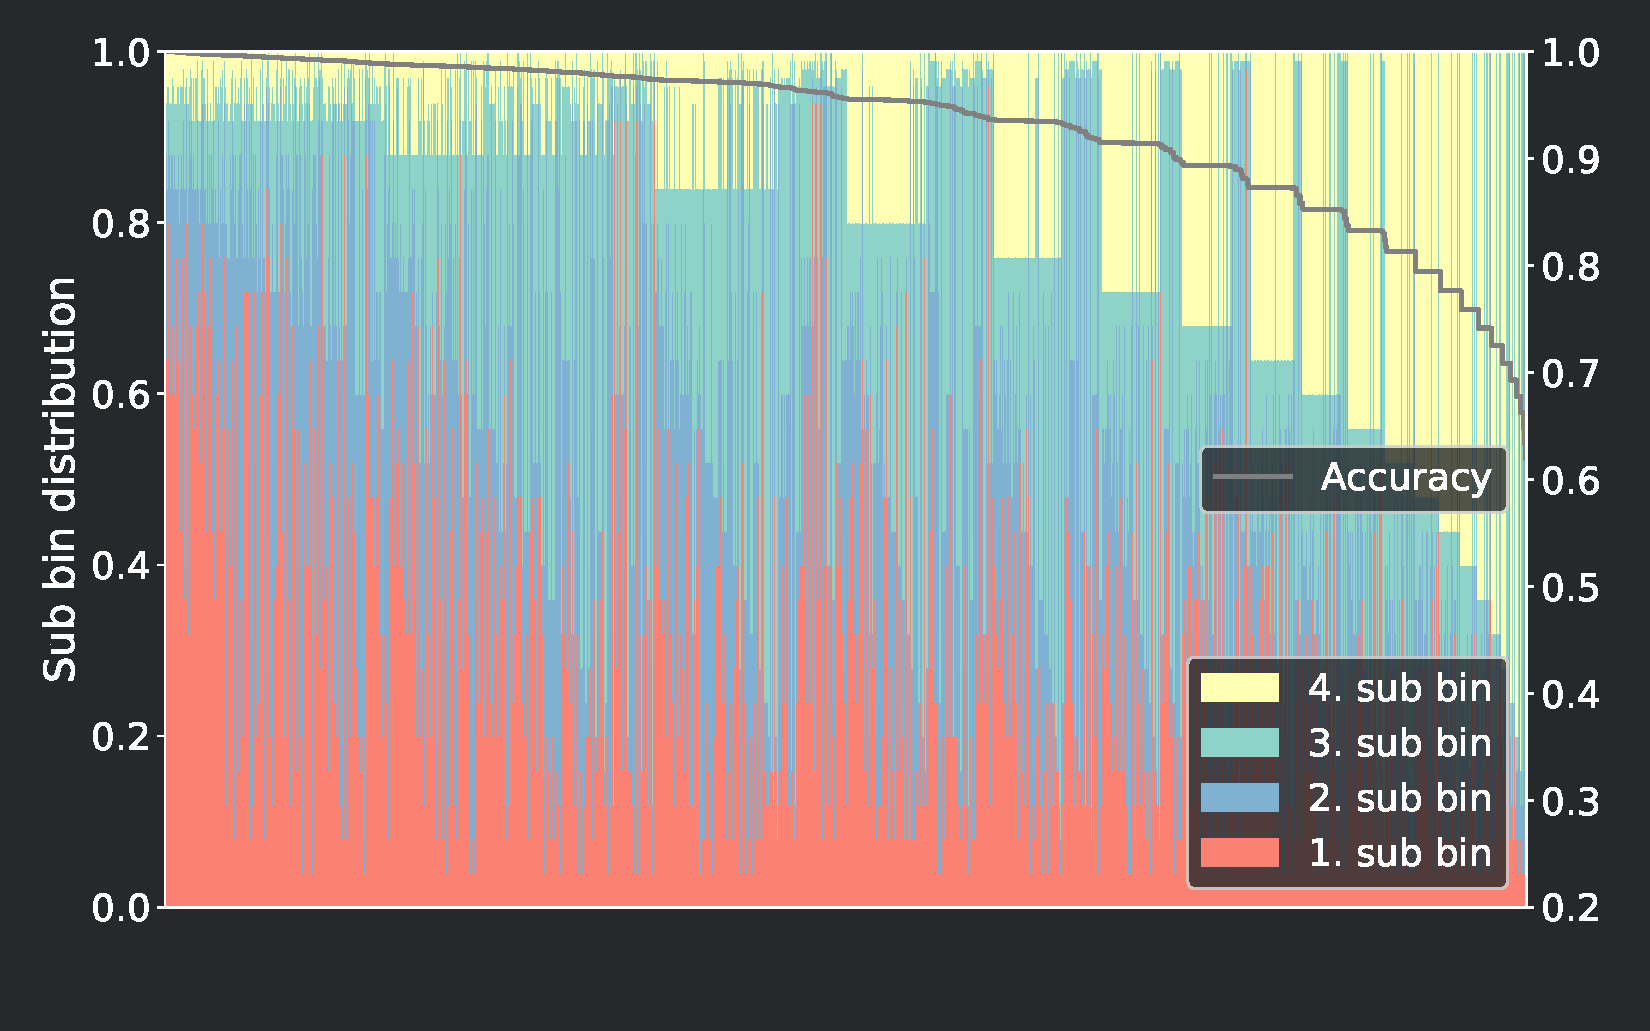
\includegraphics[width=115mm]{images/optimal_stroemgren_0_c_b}
}

\frame
{
%...................................................................................................
\note<1>[]{}
%...................................................................................................
	\frametitle{Formula: value weighted by the derivative}
	\centering
	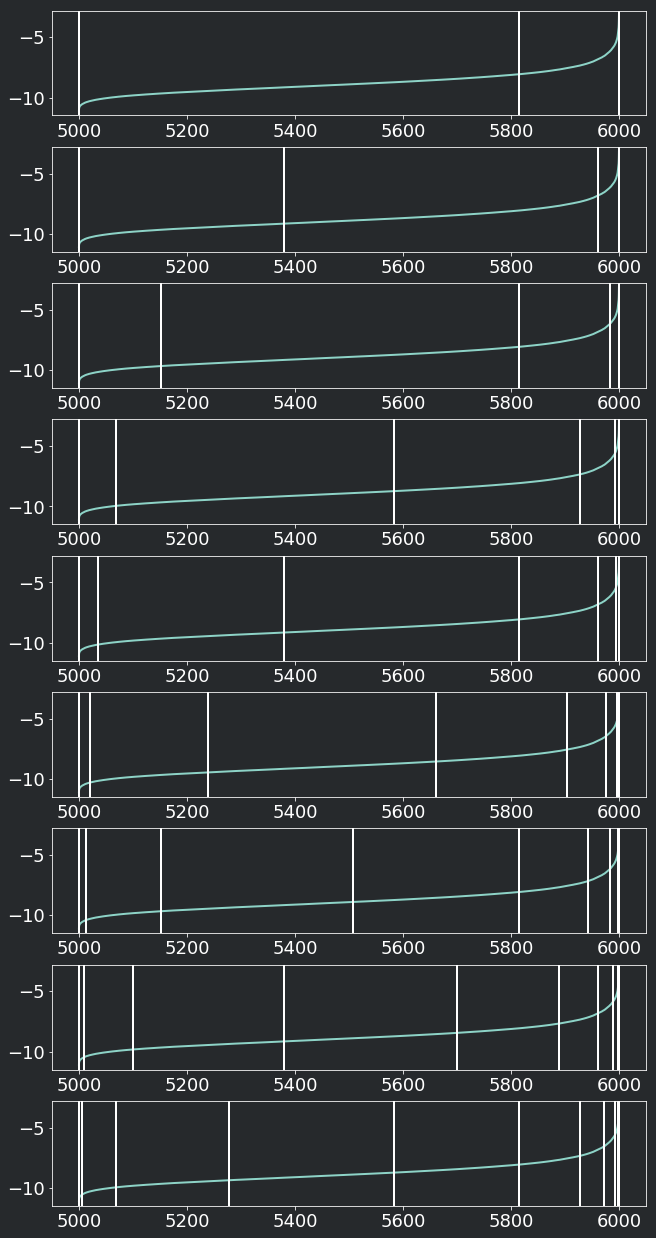
\includegraphics[width=115mm]{images/smart_sub_bins}
}
\frame
{
%...................................................................................................
\note<1>[]{}
%...................................................................................................
	\frametitle{Ascending vs descending sort}
	\centering
	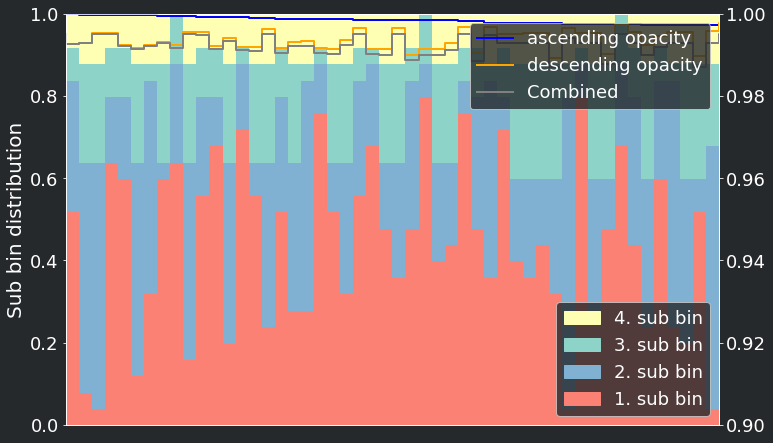
\includegraphics[width=115mm]{images/ascending_descending}
}
